%!TEX root = ../../main.tex


\begin{figure}[!htbp]
	% {\scriptsize \texthv{\textbf{(a)} Example 1}} \\
	% 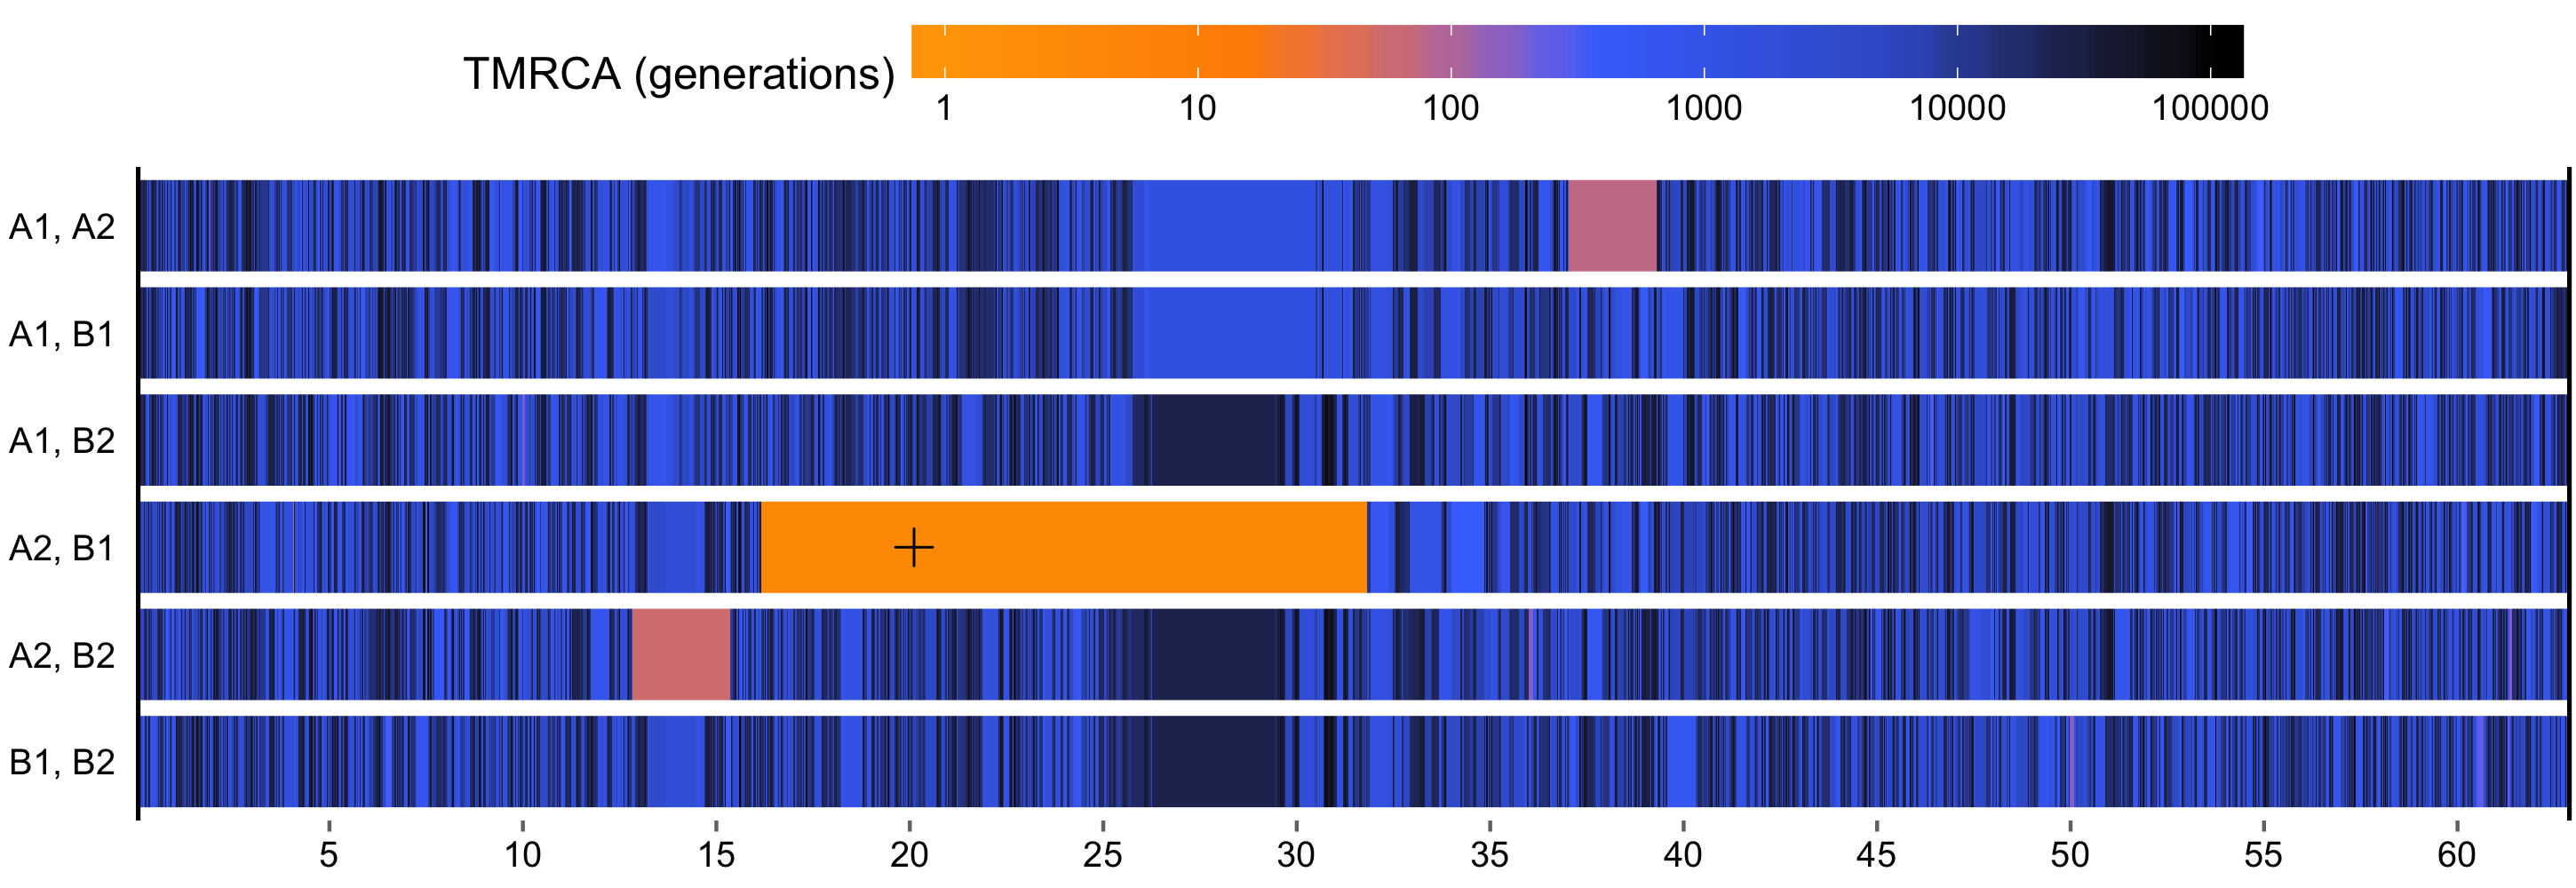
\includegraphics[width=\textwidth]{./img/ch3/full_ibd_example_A.png}
	% 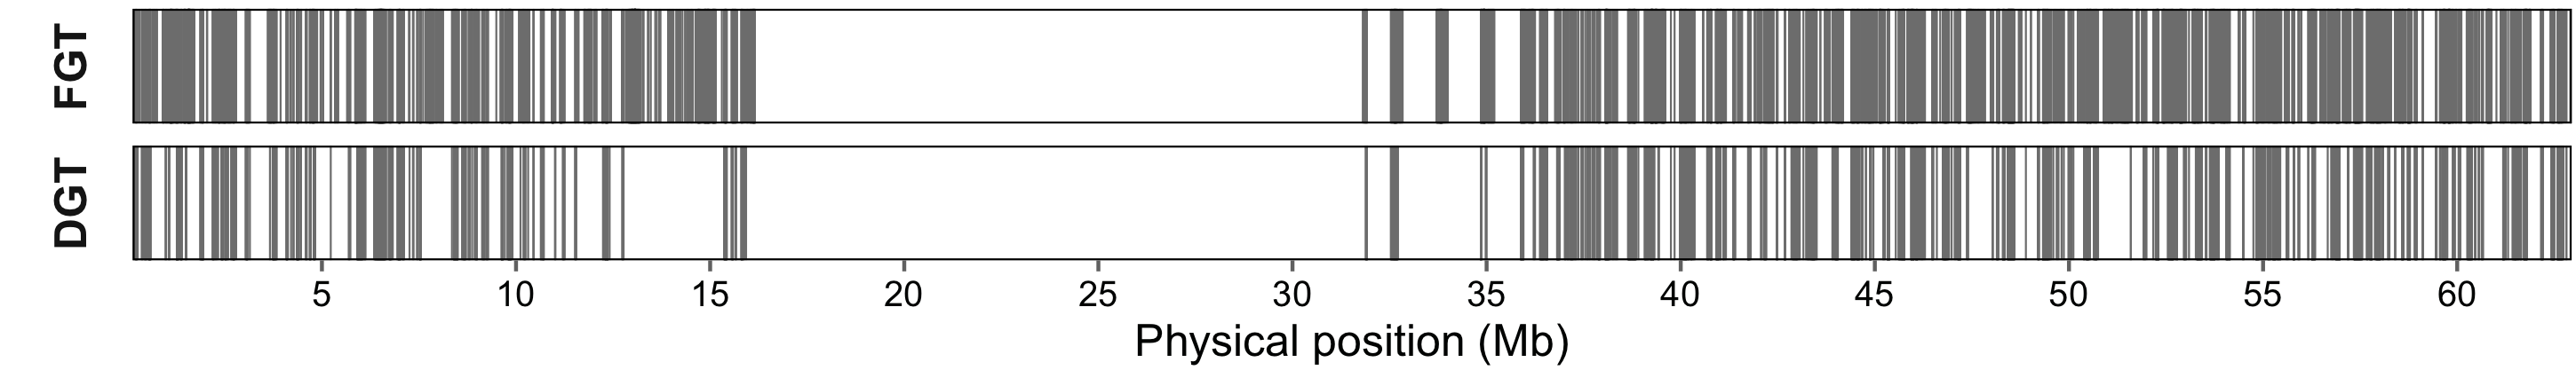
\includegraphics[width=\textwidth]{./img/ch3/full_ibd_example_B.png}
	% {\scriptsize \texthv{\textbf{(b)} Example 2}} \\
	% 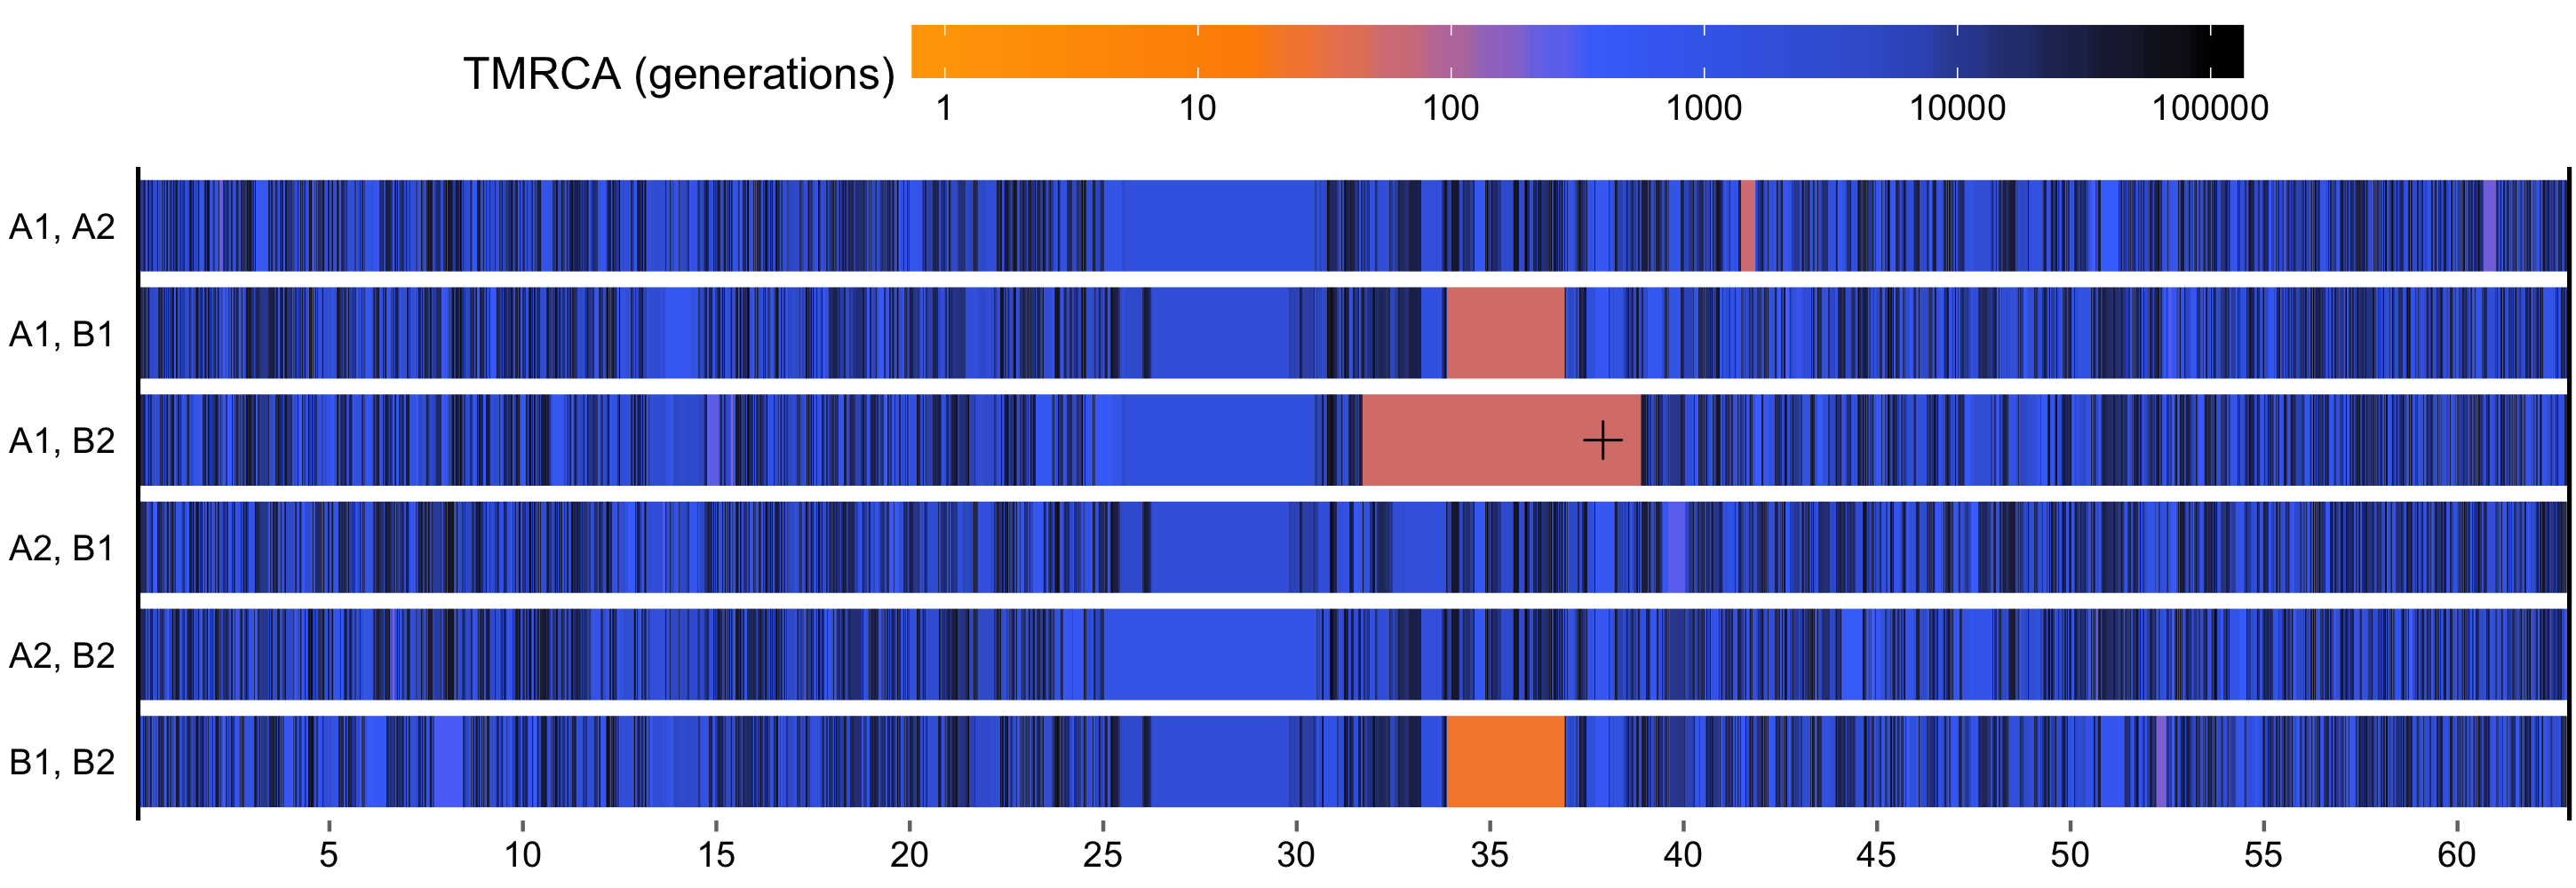
\includegraphics[width=\textwidth]{./img/ch3/full_ibd_underest_A.png}
	% 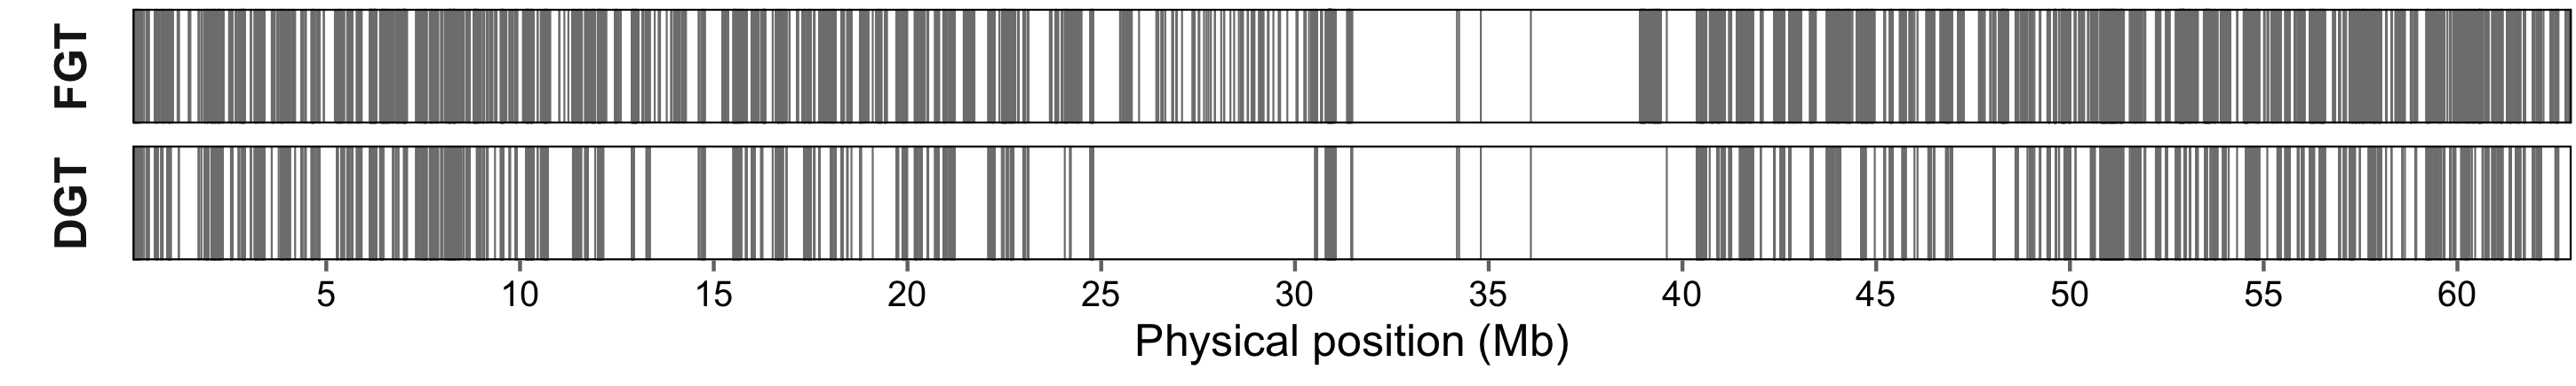
\includegraphics[width=\textwidth]{./img/ch3/full_ibd_underest_B.png}
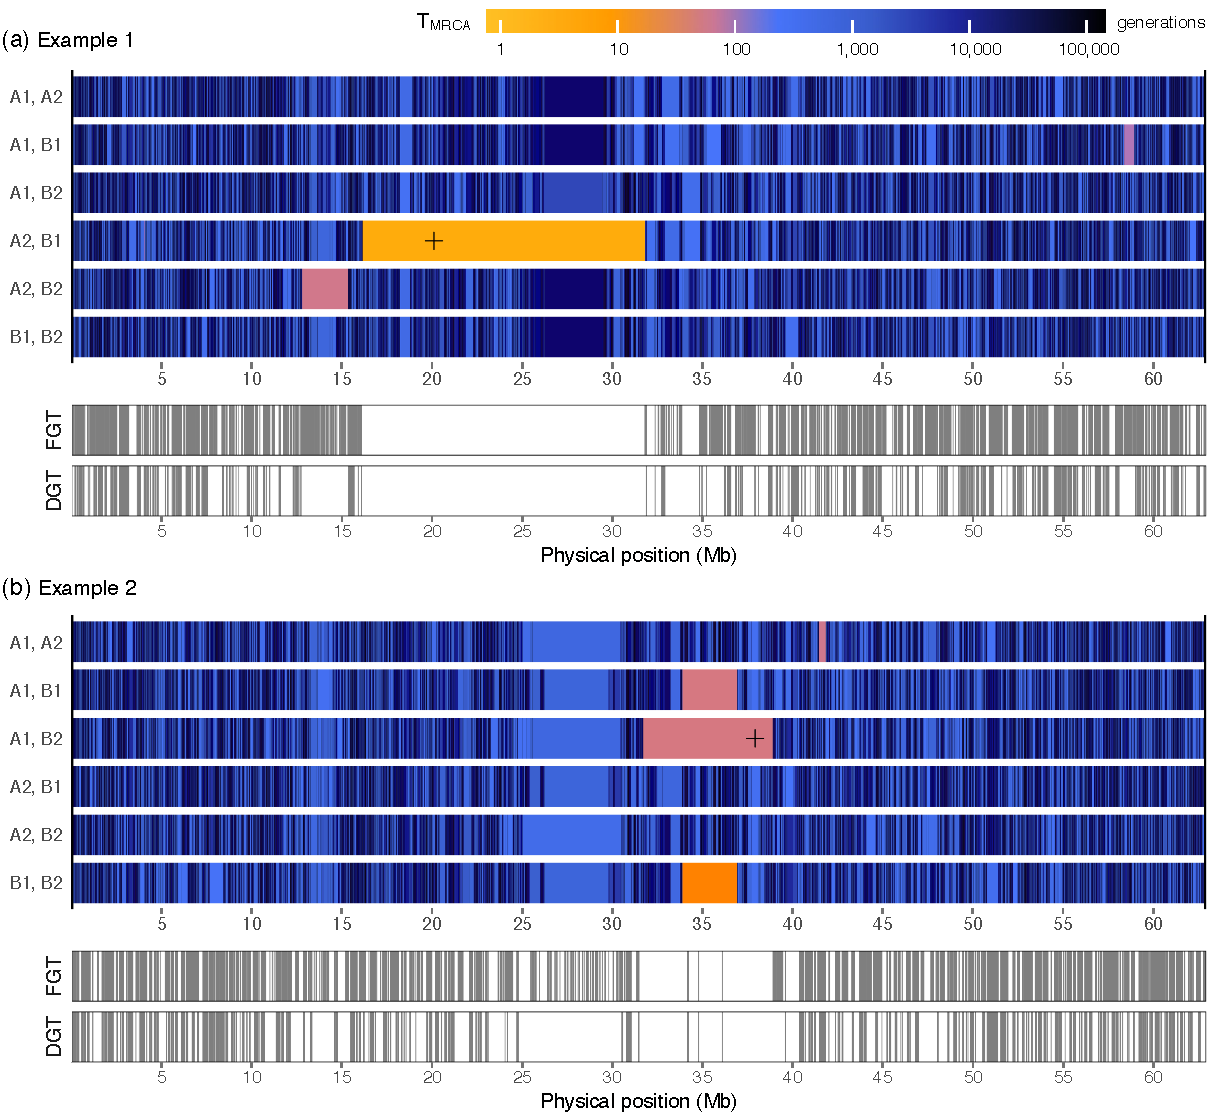
\includegraphics[width=\textwidth]{./img/ch3/full_ibd_example_reduced}
\Caption{Examples of the underlying IBD structure in each pair of four chromosomes}
{The true, underlying IBD structure is shown for each possible pair among \n{4} chromosomes in \n{2} diploid individuals; \n{2} examples are shown.
Each chromosome is labelled by its occurrence in individuals A~and~B, where chromosomes~1~and~2 are distinguished.
The ``mosaic'' of IBD segments per pair was determined from coalescent records produced in simulations using \texttt{msprime} \citep{Kelleher:2016fn}; see \cpref{sec:msprime}.
Each segment defines the region that was co-inherited from a \gls{mrca}, and is colour-coded by the number of generations separating the \n{2} chromosomes from their shared \gls{mrca} in that region.
The \emph{cross} marks the position of the focal allele in the pair that shares it.
Below, all breakpoints detected relative to the focal variant along the simulated region are indicated, using the \gls{fgt} (\emph{top}) and \gls{dgt} (\emph{bottom}).
Panel~\textbf{(a)} shows that the innermost breakpoint intervals (relative to the target position) detected in the \gls{fgt} or \gls{dgt} align closely with the true termini of the IBD segment.
The extent of overestimation appears to be negligible in relation to the length of the detected segment.
Panel~\textbf{(b)} shows that the innermost intervals are underestimated, due to an overlap of recently co-inherited haplotypes on different chromosome pairs.}
{fig:full_ibd_example}
\end{figure}
